\chapter{From Crowds: Real world perception of beauty}
\label{chap:quant_perception}

% **************************** Define Graphics Path **************************

\graphicspath{{Chapter4/plots/} {Chapter4/plots/examples/} {Chapter4/plots/GAN_examples/}}
\begin{quote}
    \textsl{Beauty is nothing other than the promise of happiness}
    -- Stendhal, \textsl{On Love}
\end{quote}

In part one, I delved deeper into the problem of quantification of perceived social support through online communities. This work showed that there are quantifiable signatures of social support in the structure and content of online communities, and these can be exploited to build models of supportive and safe interactions online, which could directly benefit persons in distress. Capturing the signatures of a subjective quantity, like the perception of social support, through the analysis of online conversations has implications on how we design better online spaces in the future. This feat is achieved through investigating networked, interacting users in communities. But the question to ask is, can unconnected agents, in large enough quantities(crowds) be use to extract signatures of perceptions. 
 
In this spirit , in the second part of my thesis, I extend the motif of perception driven design of spaces, to the offline world. The core idea is about asking a similar question, that is: \textbf{"Can we quantify the signatures of subjective perception of the real world through crowd opinions?"}. 

It has been shown through multiple studies, that the physical spaces that we use have measurable effects on our health~\cite{maas2006green,lee2011health}, our outlook towards exercise~\cite{tamosiunas2014accessibility}, health of seniors~\cite{takano2002urban} and general all round well being~\cite{gascon2015mental,nutsford2013ecological}. More importantly, all these studies point to the value of aesthetically pleasing spaces for an overall liveable city. This intuition motivates the choice of quantifying the aesthetic perception of real spaces. More so it motivates the question: Can crowd's opinion help capture a subjective quantity like the aesthetic? 
However, the question about whether an urban space is considered beautiful or not is highly subjective. To that end, we need to refine the hypothesis that we are aiming to prove. The perception of aesthetic in urban spaces are affected by location, culture, background of the crowd member and several other subjective attributes. This is why, I aim at quantifying what aspects of an urban scene "on an average" are found aesthetically pleasing to the crowds.

Research has shown that there are specific categories of urban elements that are universally considered beautiful e.g. greenery, small streets, memorable spaces, open skies~\cite{alexander1977pattern, quercia2014aesthetic,salesses2013collaborative}. These elements are those that contribute to the creation of what the urban sociologist Jane Jacobs called `urban vitality'~\cite{jacobs1961death}. 
The idea of this work is to test the quantifiable and predictive nature of these elements. In this section of my dissertation, I show that this is feasible using cutting edge deep learning and computer vision techniques and some metric design which associates meaning to the patterns in data.I use google streetview images as the source of data for photographs of urban scenes. I use crowd opinion to capture the predictive motifs of urban beauty. And I use literature drive metrics to explain and quantify the urban perception of beauty. This follows that in this chapter, I would like to answer the RQ5 of my dissertation.
 
\noindent\fbox{\begin{minipage}[t][2\height][c]{\dimexpr\textwidth-2\fboxsep-2\fboxrule\relax}
        \textbf{RQ5} \textsl{Can crowdsourcing and machine learning help us quantify how humans perceive beauty in urban settings?}   
\end{minipage}}
\\


\section{Related Work}
\label{sec:related}
The problem of designing better cities, has been a on going obsession for various fields. A lot of work was done in the past in just understanding the concept of good , liveable cities. One of the most prominent figure in the campaign to re-vitalize our cities was Jane Jacobs in the late 50s.  Jacobs's seminal work on urban vitality~\cite{jacobs1961death} discusses the idea of how a design of a city might be the driving reason behind how urban vitality thrives. Christopher Alexander was another such prominent voice who in his book undertook a cataloguing exercise  of typical ``patterns'' of good urban design~\cite{alexander1977pattern}. This effort showed that certain patterns of placements of roads, trees, walkways, parks and areas of social interactions are highly crucial in promoting a thriving social environment. In the fields of psychology, environmental design and behavioral sciences, research has studied the relationship between urban aesthetics~\cite{real2000classification} and a variety of objective measures  (e.g.,  scene complexity~\cite{kaplan1972rated}, presence of nature~\cite{kaplan1989experience}) and subjective ones (e.g., people's affective responses~\cite{ulrich1983aesthetic}). As mentioned before, the relation between greenery and the design of spaces around us has been linked with  measurable effects on our health~\cite{maas2006green,lee2011health}, our outlook towards exercise~\cite{tamosiunas2014accessibility}, health of seniors~\cite{takano2002urban} and general all round well being~\cite{gascon2015mental,nutsford2013ecological}.

With the premise of all this, it is worth exploring the literature to understand how different fields are working towards using this relation between the humans and the spaces they occupy.
%\mbox{}\\
\vspace{4pt}\noindent
\textbf{Ground truth of urban perceptions.} So far, the most detailed studies of perceptions of urban environments and their visual appearance have relied on personal interviews and the observation of city streets: for example, some researchers relied on annotations of video recordings by experts~\cite{sampson04seeing}, while others have used participant ratings of simulated (rather than existing) street scenes~\cite{lindal2012}. The Web has recently been used to survey a large number of individuals. Place Pulse is a website that asks a series of binary perception questions (such as `Which place looks safer [between the two]?') across a large number of geo-tagged images~\cite{salesses2013collaborative}. In a similar way, Quercia \emph{et al.} collected pairwise judgments about the extent to which urban scenes are considered quiet, beautiful and happy~\cite{quercia2014aesthetic} to then recommend pleasant paths in the city~\cite{quercia2014shortest}. They were then able to analyze the scenes together with their ratings using image-processing tools, and found that the amount of greenery in any given scene was associated with all three attributes and that cars and fortress-like buildings were associated with sadness. Taken all together, their results pointed in the same direction: urban elements that hinder social interactions were undesirable, while elements that increase interactions were the ones that should be integrated by urban planners to retrofit cities for happiness. Urban perceptions translate in concrete outcomes. Based on 3.3k self-reported survey responses,  Ball et al.~\cite{ball2001perceived} found that urban scenes with positive aesthetics properties  not only are visually  pleasurable but also promote walkability. Similar findings were obtained by Giles et al. \cite{giles2005increasing}.
%\mbox{}\\

\vspace{4pt}\noindent
\textbf{Deep learning and the city.} Computer vision techniques have increasingly become more sophisticated. Deep learning techniques, in particular, have been recently used to accurately predict urban beauty~\cite{dubey2016deep,seresinhe2017using}, urban change~\cite{naik2017computer}, and even crime~\cite{DeNadai16,arietta2014city}.  Recent works have also showed the utility of deep learning techniques in predicting house prices from urban frontages~\cite{frontage}, and from a combination of satellite data and street view images~\cite{law2018take}.

\vspace{4pt}
To sum up, a lot of work has gone into collecting ground truth data about how people tend to perceive urban spaces, and into building accurate predictions models of urban qualities. This trove of human annotated ground truths about urban spaces is vital in understanding human perception at scale. In this chapter we would look at a way to transfer the collective perception of humans in to a machine learning model. Doing so we would validate whether machine learning models can actually capture the subjective perceptions of people. 

\section{The Data}

\label{Sec:dataset}
To begin with, we need highly curated training data with labels that reflect the crowds consensus on beauty. Unfortunately, it is difficult to get data where thee is a consensus on of the crowds on an absolute value of beauty. However there are datasets available where crowds have voted on pairwise comparisons of urban images for their relative beauty. The two most prominent examples are from MIT media lab~\cite{dubey2016deep} called the place pulse and from Bell labs~\cite{quercia13maps}. 

\begin{figure}
   \centering   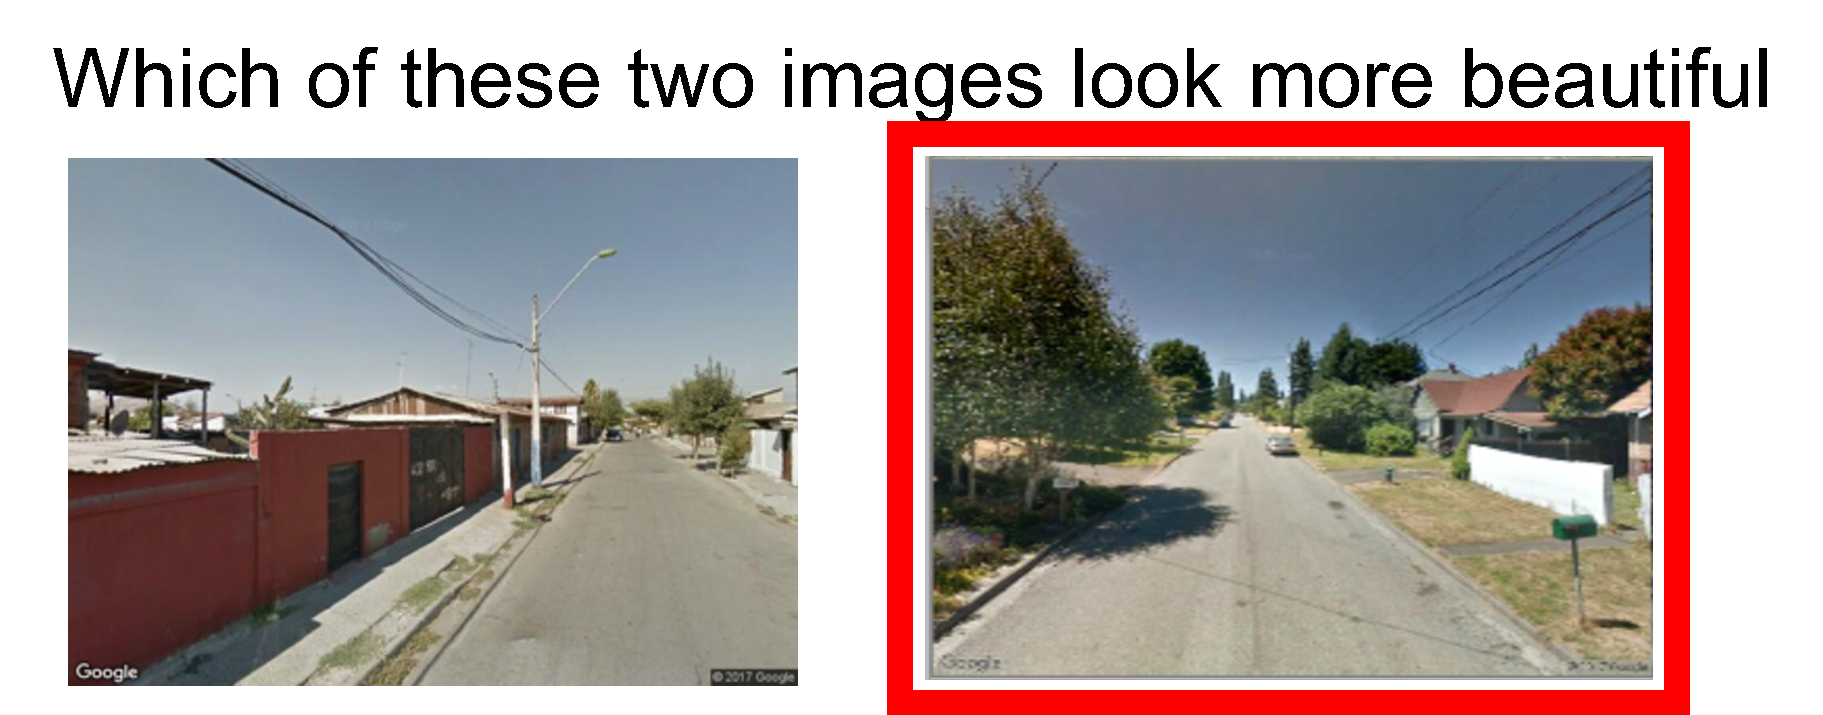
\includegraphics[width=\columnwidth]{Pairwise.pdf}
   \caption{Example of a paiwise comparison, where a user is asked to choose the more beautiful among the two.}
   \label{fig:pairwise}
\end{figure}

We start with the  Place Pulse dataset that contains 100k Google Street Views across 56 cities around the world~\cite{dubey2016deep}. The voting on these scenes is taken in the form of a gamified interface, where two random images from this set are shown, and the participant is asked to choose the more beautiful of the two. The interface looks similar to Figure \ref{fig:pairwise}, where by one would preferentially end up choosing the image on the right, due to its objectively superior aesthetics as compared to the one on the left. Over the course of time, they gather votes on more than 1.2 pairwise comparisons, distributed  across 100k images, given my more than 81k participants.
This process, still does not solve the problem of obtaining an annotated dataset of beautiful and ugly looking urban neighbourhoods. For that to happen, we first need to translate these comparisons in to some form of an ordinal ranking of images.

\subsection{Partitioning the data}
To solve the problem of annotating images in terms of beauty, we need to have , at the very least, a sense of relative ranking in terms of most popularly voted to be beautiful to the least. This approach would not quantify beauty in the absolute sense, but in terms of relative consensus, provided we have enough pair wise votes. 
 
\begin{figure}[t!]
    \centering
    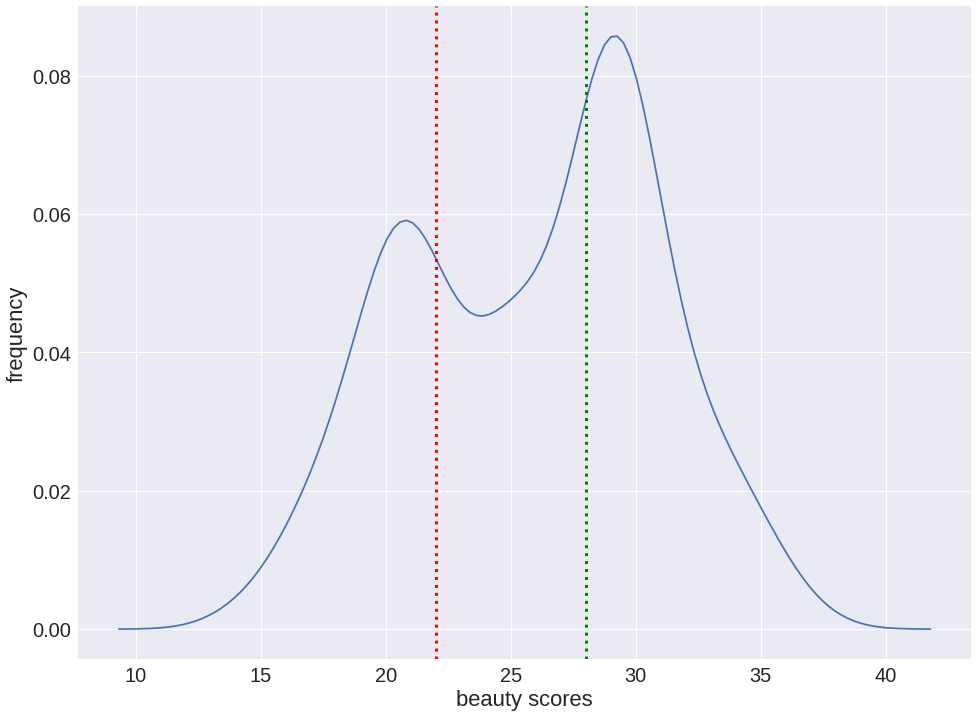
\includegraphics[width=0.7\columnwidth]{Trueskill.png}
    \caption{Frequency distribution of beauty scores. The red and green lines represent the thresholds below and above which images are considered ugly and beautiful. Conservatively, images in between are discarded.}
    \label{fig:Trueskill}
\end{figure}
To solve the problem of transforming the pairwise voting of the crowd into relative ordinal ranking, we use a popular Bayesian algorithm, used in several multiplayer gaming systems to order leader boards called TrueSkill~\cite{herbrich2007trueskill}. This algorithm works by first initializing all the players (which in our case are urban street view images) with equal ``skill'' (which in our case implies a relative sense of beauty).
The algorithm then assumes competitions among the players in a 1-on-1 fashion. In the case of our work, these competitions are the pairwise votes. Each victory results in addition of some ``skill''(beauty) in the victor player's profile (street-view image) and reduction in ``skill'' in the loser's profile. The more skillful the opponent, the higher the rewards in update of one's skill. With enough average number of competitions played by each player, a steady state order of skilled players emerges. For our dataset, we initialize all images with a ``skill'' level of 25 and a variance of 3, which signifies the uncertainty in the skill level. This uncertainity would drop, as more competitions are won or lost by any given image. For the sake of accuracy and stability, we filter only the images which have more than 8 votes on them. This reduces our usable dataset from 100k images to just over 20k. But having more than 8 votes, results in a steady state bi-modal distribution of skills as shown in Figure \ref{fig:Trueskill}. This allows us to order the streetview images in an ordinal rank based on relative beauty as seen in Fig \ref{fig:trueskill_example}. 

\begin{figure}[t!]
    \centering
    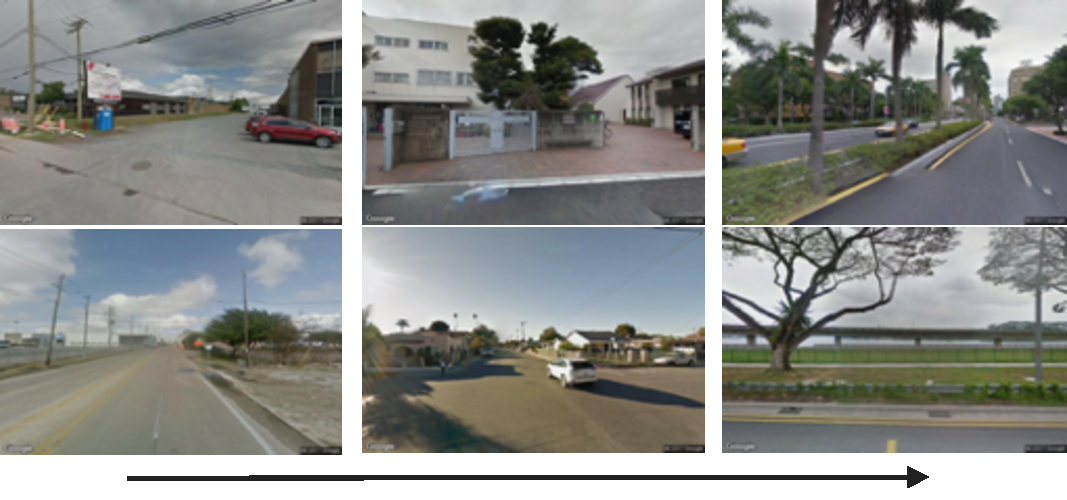
\includegraphics[width=\columnwidth]{SkillSorting.pdf}
    \caption{Sample pairs of street view images ordered by lowest final skill rating on the left to highest on the right. }
    \label{fig:trueskill_example}
\end{figure}
Despite having a consensus on the ordering of most of the images, we still end up with some images near the initialized skill level of 25. This means the skills of these images have not been decisively updated through the voting data. To work around these borderline cases, we partition the distribution of images along two margins in the trueskill space. We conservatively select all images with a Trueskill value less than 22 and assign them to the ugly set of images. We then select all the images with the trueskill value above 28, and assign them to the beauty bin. We arrive at these values of partitioning, by conservatively evaluating how many images we are left with, without polluting the data with borderline cases.


\subsection{Augmenting the data}
\begin{figure}[t!]
    \centering
    \subfloat[]{
        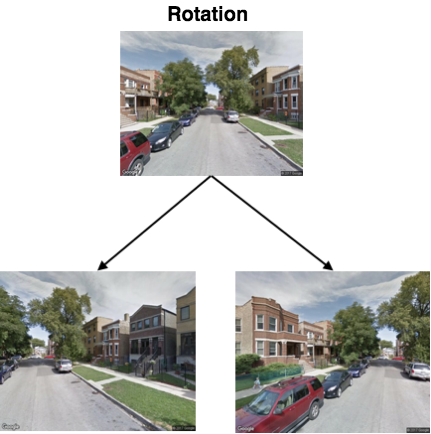
\includegraphics[width=0.5\textwidth, height = 8cm ]{rotationalSim.png}
        \label{fig:rotSim}
    }
    \subfloat[]{
        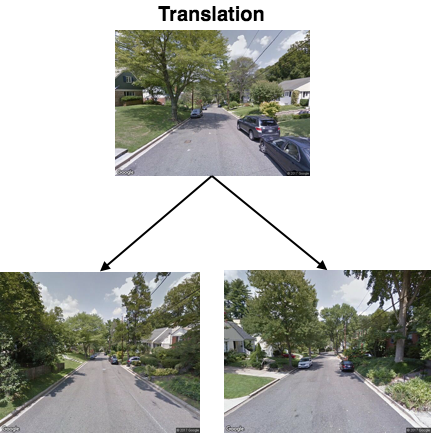
\includegraphics[width=0.5\linewidth, height = 8cm ]{transSim.png}
        \label{fig:transSim}
    }
    \caption{Two types of augmentation: (a) rotation of the Street Views camera (based on rotation); and (b) exploration of scenes at increasing distances (based on translation).}
\end{figure}
Partitioning of the data after evaliating the Trueskill scores on images is a lossy process. By the time we filter images along minimum number of votes, and based on their trueskill scores, we are left with 15,000 street-view images. It has been a well known problem in the area of deep learning, that the algorithm's performance is often limited by the amount of clean curated data available to train on. Another real danger of training on limited data is the phenomenon of over fitting. Overfitting happens when the model under consideration is reasonably complicated with millions of parameters, but the data used to train it is not sufficient to generalize the model's inference. In such cases, the model over fits to the training dataset whereby the model memorises the training data, to reduce the training error. But this model is doomed to perform poorly on a generalized set of data. To avoid this particular set of problems, I needed a way to enrich the current high confidence set of steetview images. The enrichment needs to be such that we do not add noise to the dataset, but at the same time increase the diversity of the kind of samples the model is supposed to learn. This means we need more images which are similar but not identical to the two partitions. 

The solution I develop involves two approaches. First, we feed each scene's location into the Google Streetview API to obtain the snapshots of the same location at different camera angles\footnote{Google streetview API allows the users to set the bearing and heading of the mast camera, used to acquire the image} (i.e., at $\theta \in {-30^{\circ}, -15^{\circ} , 15^{\circ} , 30^{\circ} }$). We assume that any image taken as a variant of a beautiful image at different angles of rotations can safely inherit the label of ``beauty'' since the field of view only changes by $+- 30^\circ $. With this simple (yet conservative) assumption we are able to immediately inflate our dataset by up to a factor of 5.
However, the resulting dataset is still too small for robust training. Therefore, again, we feed each scene's location into the Google Streetview API, but we now do so to obtain other scenes at  distance $d \in \{10,20,40,60\}$ meters.  This will greatly expand our set of scenes, but it might do so at the price of introducing scenes whose beauty scores have little to do with the original scene's. 
This addition of noise may have an adverse effect on the deep learning algorithm's performance for detecting beauty. 
This addition of translational data, could be done using some heuristics. Imagine a scene $I$ translated in space by 10 meters. The newly acquired scene $I_{10}$, may be useful in our augmented dataset \textit{iff} the translated scene $I_{10}$ is visually ``similar'' to the original scene $I$. The same heuristic metric can be used to either accept or reject any image $I_{m}$ translated by $m$ meters, into the augmented dataset. 
For this heuristic test to work, we first need to device a way to compute the ``similarity'' measure between two images $I$ and $I_{m}$. 
One well known way to evaluate image ``similarity'' is by represent them in a high dimensional features space, obtained from a pre-trained neural network. This is done by using the activations of a the fully connected layer of a trained convolutional neural network during a forward pass~\cite{babenko2015aggregating,Lin_2015_CVPR_Workshops,varga2016fast}. These activations are then treated as vectors in $R^N$ euclidean space, such that they follow the distance and angle metrics. This allows comparison of images along a similarity metric simply by comparing the distances between their feature vectors. For the sake of similarity of application, we use the best performance version of a pre-trainied PlacesNet deep learning model~\cite{zhou2014learning}. PlasesNet was trained on streetview images, and is trained with the end goal of classifying streetview images into scene types, such as a beach, highway, garden etc. We represent the two scenes $I$ and $I_m$ with visual features derived from the \textsl{FC7} layer of PlacesNet and compute the similarity between the two corresponding feature vectors using L1 norm. 
For all scenes$I_m$ at increasing distance $m \in \{10,20,40,60\}$ meters,  we take only those whose similarity scores with the original scene is above a threshold. In a conservative fashion, we choose that threshold to be the median similarity between rotated and original scenes (those of the first augmentation step). This assures that the translated images are at the very least as similar to the original, as the rotated images.
\subsubsection{Which scenes are more suitable for translation?}
\begin{figure}[t!]
    \centering
    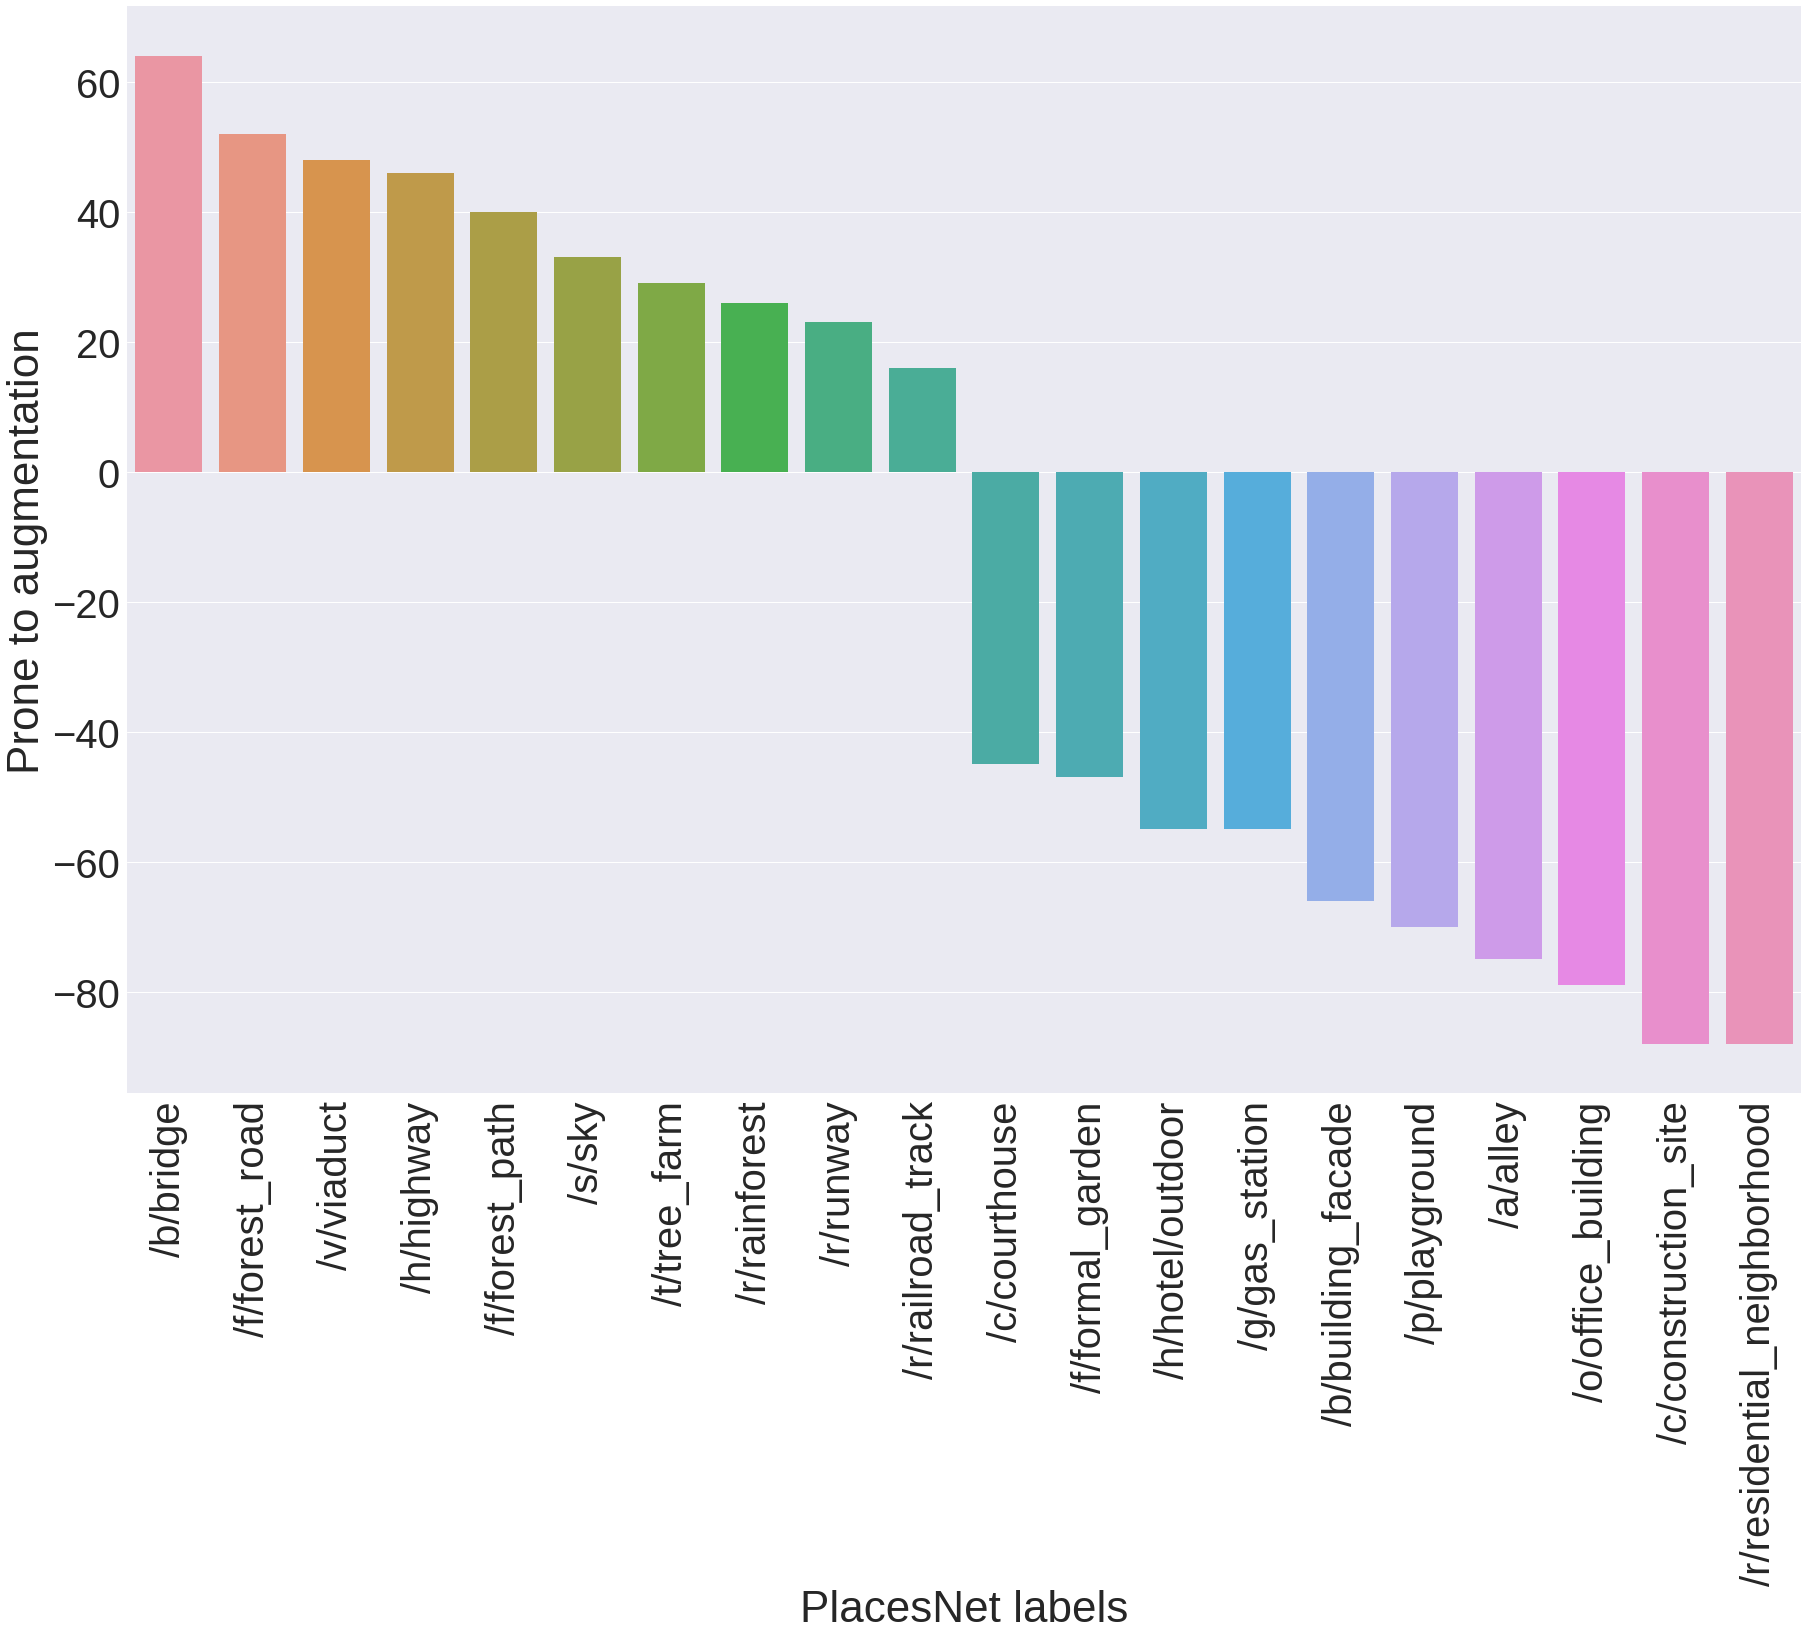
\includegraphics[width=\columnwidth]{SimilarityPlacesPrevalence.png}
    \caption{The types of scene that have greater propensity to be correctly augmented with similar scenes at increasing distances.}
    \label{fig:augmentationSimilarity}
\end{figure}
To make sure this additional augmentation has not introduced any unwanted noise, we consider  two sets of scenes: one containing those that have been taken during this last step, i.e., the one with high similarity to the original scenes:(\emph{taken-set}), and the other containing those that have been filtered away because their similarity metric went above the threshold:(\emph{filtered-set}). Each scene is then scored with PlacesNet~\cite{zhou2014learning} and is represented with the five most confident scene labels, as per the original output of the model . We then aggregate labels at set level by computing each label's frequency on the \emph{taken-set} 
and on the \emph{filtered-set}. Finally, we characterize each label's propensity to be correctly augmented as: 
$ \textrm{prone}(label)= fr(label,\textrm{\emph{taken-set}}) - fr(label,\textrm{\emph{filtered-set}}).$
This reflects the extent to which a scene with a given scene label is prone to be augmented or not, according to our decided threshold method. From Figure~\ref{fig:augmentationSimilarity}, we find that, as one would expect, scenes that contain high amount of visual continuity over long stretches such as highways, fields and bridges can be augmented at increasing distances while still showing resemblances to the original scene. By contrast, scenes that contain peculiar features with smaller continuity such as gardens, residential neighbourhoods, plazas, and skyscrapers cannot be easily augmented. These scene types also tend to be found in high density parts of the city in which visual diversity within short distances might well be experienced. 

\section{Building a beauty Classifier}

\begin{figure*}[t!]
    \centering
    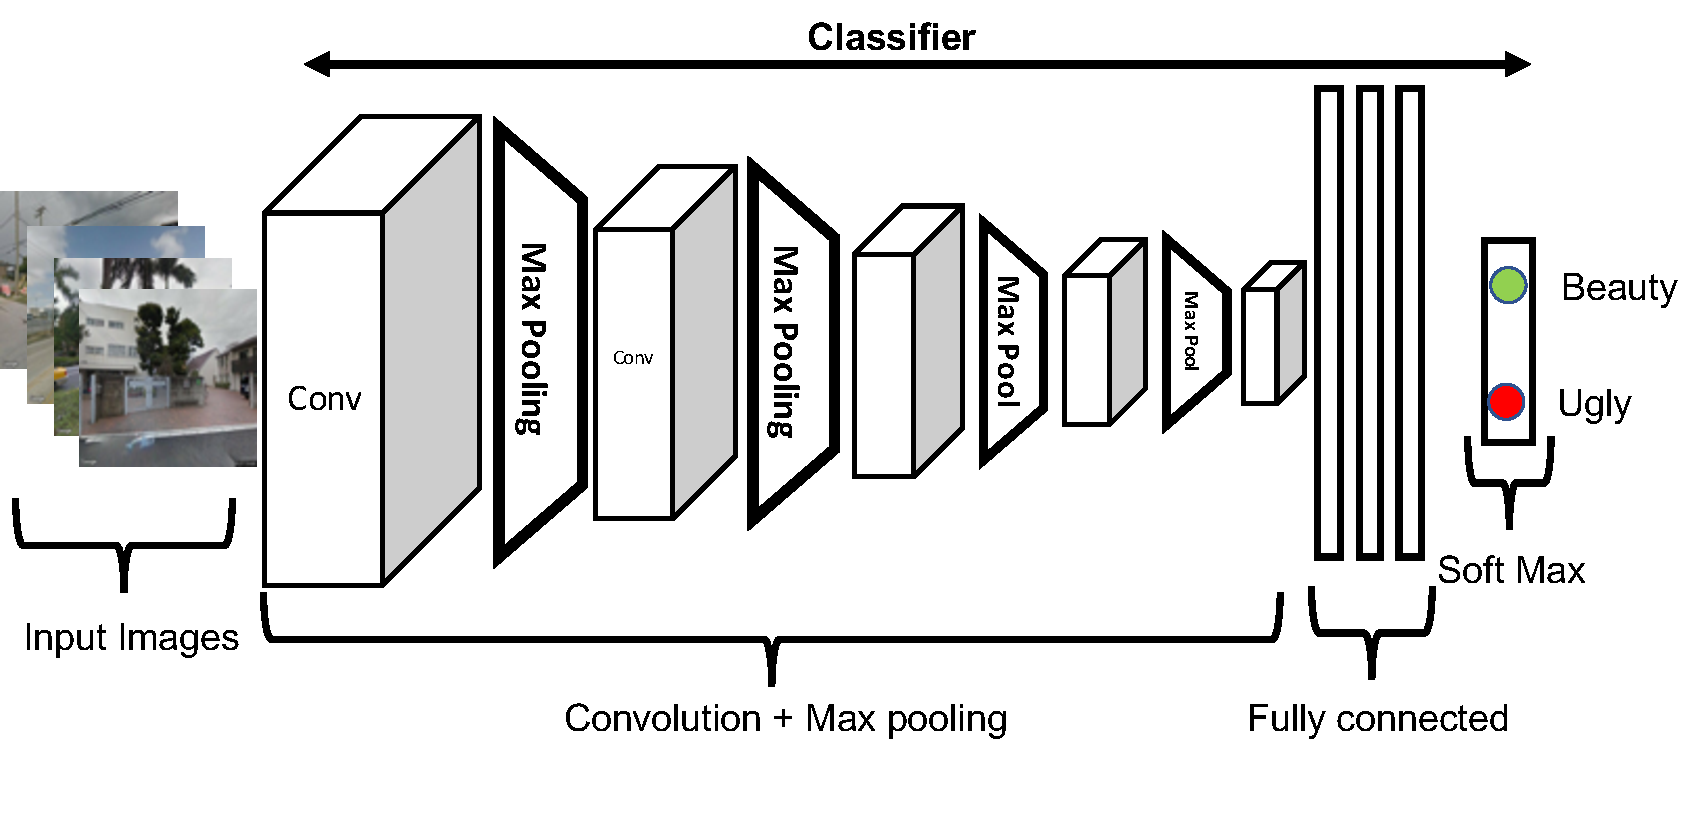
\includegraphics[width=\columnwidth]{Classifier_arch.pdf}
    \caption{}
    \label{fig:classifier_arch}
\end{figure*}

\label{sec:framework}
\begin{table}[ht!]
    \centering
    \begin{tabular}{|c|c|}
        \hline
        \textbf{Augmentation} & \textbf{Accuracy (Percentage)}\\
        \hline
        None & 63 \\
        \hline
        Rotation  & 68 \\
        \hline
        Rotation + Translation  & 64 \\
        \hline
        Rotation + Conservative Translation & 73.5 \\
        \hline
    \end{tabular}
    \caption{Percentage accuracy for our beauty classifier trained on differently augmented sets of  urban scenes.}
    \label{tab:classifier}
    \vspace{-10mm}
\end{table}

Having this highly curated set of labeled urban scenes, we are now ready to train classifier $C$ with labels reflecting our beauty assessments. The challenge here is to understand if a deep learning model is able to capture the essence of something as subjective as \textbf{perceived urban beauty}.

As for classifier $C$, we use the CaffeNet architecture, a modified version of AlexNet~\cite{krizhevsky2012imagenet,szegedy2015going} as seen in Figure \ref{fig:classifier_arch}. This has a conventional architecture with 5 convolutional layers; interleaved with  max pooling and normalization layers; and terminated by: \emph{(i)} three 4096 dimensional fully connected layers interleaved with dropout layers~\cite{srivastava2014dropout} (the dropout ratio is set to 0.5 to prevent over-fitting), and \emph{(ii)} by a Softmax layer that classifies the input image into one of two classes of beautiful(1) and ugly(0).  

Having $C$ at hand, we now turn to training it. The training is done on a 70\% split of the data, and the testing on the remaining 30\%. All this is done on increasingly augmented sets of data. We start from our 20k images and progressively augment them with  the snapshots obtained with the 5-angle camera rotations, and then with the exploration of scenes at increasing distance $d \in \{10,20,40,60\}$ meters. The idea behind this data augmentation is that the model's accuracy should increase with increasing levels of augmentation. Indeed it does (Table~\ref{tab:classifier}): it goes from 63\% on the set of original scenes to a value as high as  73.5\% on the set of fully augmented scenes, which is a notable increase in accuracy for this type of classification tasks. Furthermore, our results match previous ones: for example,  Dubey et.al's~\cite{dubey2016deep}  model showed an accuracy of 70\%, which is comparable to ours. 
The comparable, and at times better, performance of this classifier with respect to the baseline shows that 1) the notion of subjective beauty can be learn't from a crowd's participation and 2) the novel method of augmenting data, can make deep learning better accessible when the data is sparse and of urban nature.

\section{Implication of a beauty classifier}
In this chapter, we found that using a crowd based pooling of opinions of urban beauty, we can make measurable progress towards quantifying the aesthetic in the context of urban scenes. This too can be done at scale, with a novel way of augmenting sparse datasets. However, just capturing the perception is not enough to make any meaningful contribution towards the urban science. A lot of work has been put in understanding the impact of the urban aesthetic of citizen's health, well being, economical vitality etc. The unanimous consensus points to the fact that cites and their compositions deeply affect our health and well being. 
At this juncture it is more valuable to first understand if the notion of beauty captured by our deep learning model is analogues to that perceived by real humans. If that is indeed the case, it is worth understanding what aspects of an urban scene are predictive of the perceived beauty. This shall be of immense value to the practitioners of urban design, architecture and urban activism.

In the next chapter, we would explore exactly that. The guiding question is, can the learnt representation of urban beauty be utilized to understand the predictive motifs of urban design for beauty? Can these insights be used in a constructive way to improve existing urban scenes ? And finally, can such a framework be useful to the cause of urban design ? 


